\documentclass[a4paper,12pt]{article}
\usepackage[utf8]{inputenc}
\usepackage{fontspec} 
%\XeTeXlinebreaklocale "zh" 
%\XeTeXlinebreakskip = 0pt plus 1pt 
%\setmainfont[Mapping=tex-text]{DejaVu Serif} % rm
\usepackage{graphicx}
\usepackage[a4paper]{geometry}
%\setlength{\textwidth}{5in}
%\setlength{\hoffset}{0.6in}
%header
\usepackage{fancyhdr}
%math package
\usepackage[fleqn]{amsmath}
%\usepackage{amsmath,amssymb}
%code package
%\usepackage{minted}
\usepackage{listings}
\usepackage{minted}
\usepackage[lined,boxed]{algorithm2e}


\newcommand{\horrule}[1]{\rule{\linewidth}{#1}} 
\title{	
\normalfont \normalsize \vspace{-13em} % Your university, school and/or department name(s)
\horrule{1pt} \\[0.5cm] % Thick bottom horizontal rule
\huge Neural Network
\\ % The assignment title
\vspace{1em}
\large Assignment 1
\horrule{2pt} \\[0.5cm] % Thick bottom horizontal rule
}
\author{Zhao Shenjian 5110309748}
\date{}
\pagestyle{fancy}
\rhead{Two Spiral Problem}


\begin{document}   
\maketitle
\thispagestyle{empty}
\setcounter{page}{1}
\section*{Part I: Back-propagation Algorithms}
  \subsection*{1.1 On-line learning} 
  \subsubsection*{Case 1: Neuron j is an Output Node} 
  \paragraph{} Because I don't have enough time to write the entire derivation, I only write the final result. It's definitely right, because I have check
  it using my program.\\
  \begin{align*}
    \delta_{j}(n) &= e_j(n)f^{\prime}_j(net_j) =  e_j(n)f(net_j)(1-f(net_j))\\
     \Delta u_{ji}(n) &= \eta \delta_j(n)x^{2}_i(n) \\
     \Delta v_{ji}(n) &= \eta \delta_j(n)x_i(n) \\
     \Delta b_j(n) &= \eta \delta_j(n)
  \end{align}

  $f$ is sigmoid activation function, $net_j = \Sigma  u_{kji}x^{2}_{k-1,i} + v_{kji}x_{k-1,i} + b_{kj}$

  \subsubsection*{Case 2: Neuron j is a Hidden Node} 
  \begin{align*}
    \delta_{j}(n) &= f^{\prime}_j(net_j) \varSigma_{k}(\delta_{k}(n)(2u_{kj}(n)x_j + v_{kj}(n)))\\
     \Delta u_{ji}(n) &= \eta \delta_j(n)x^{2}_i(n) \\
     \Delta v_{ji}(n) &= \eta \delta_j(n)x_i(n) \\
     \Delta b_j(n) &= \eta \delta_j(n)
  \end{align}
  
  
  
  \subsection*{1.2 Batch learning}
  \subsubsection*{Case 1: Neuron j is an Output Node} 
   \begin{align*}
    \delta_{j}(n) &= e_j(n)f^{\prime}_j(net_j) =  e_j(n)f(net_j)(1-f(net_j))\\
     \Delta u_{ji}(n) &= \cfrac{\eta}{N} \Sigma_n(\delta_j(n)x^{2}_i(n)) \\
     \Delta v_{ji}(n) &= \cfrac{\eta}{N} \Sigma_n(\delta_j(n)x_i(n)) \\
     \Delta b_j(n) &= \cfrac{\eta}{N}\Sigma_n\delta_j(n)
  \end{align}
  
   \subsubsection*{Case 2: Neuron j is a Hidden Node} 
    \begin{align*}
    \delta_{j}(n) &= f^{\prime}_j(net_j) \varSigma_{k}(\delta_{k}(n)(2u_{kj}(n)x_j + v_{kj}(n)))\\
    \Delta u_{ji}(n) &= \cfrac{\eta}{N} \Sigma_n(\delta_j(n)x^{2}_i(n)) \\
     \Delta v_{ji}(n) &= \cfrac{\eta}{N} \Sigma_n(\delta_j(n)x_i(n)) \\
     \Delta b_j(n) &= \cfrac{\eta}{N}\Sigma_n\delta_j(n)
  \end{align}
  
 \section*{Part II: C++ implementation}
 \paragraph{}In order to master every detail of neural network and gain efficiency, I use c++ to solve this problem.
 The source code is in src folder. Please read the README to build and run the program. 
 \paragraph{}However I use matlab to plot the result image, it doesn't matter.

 \section*{Part III: Test results}
 \subsection*{3.1 Correctness}
  \paragraph{}
 First to say, my result is correct. The misclassification is 0 for both online learning and batch learning. The following two pictures
 shows the results.

 
 \begin{figure}[h]
\centering
\subfigure{
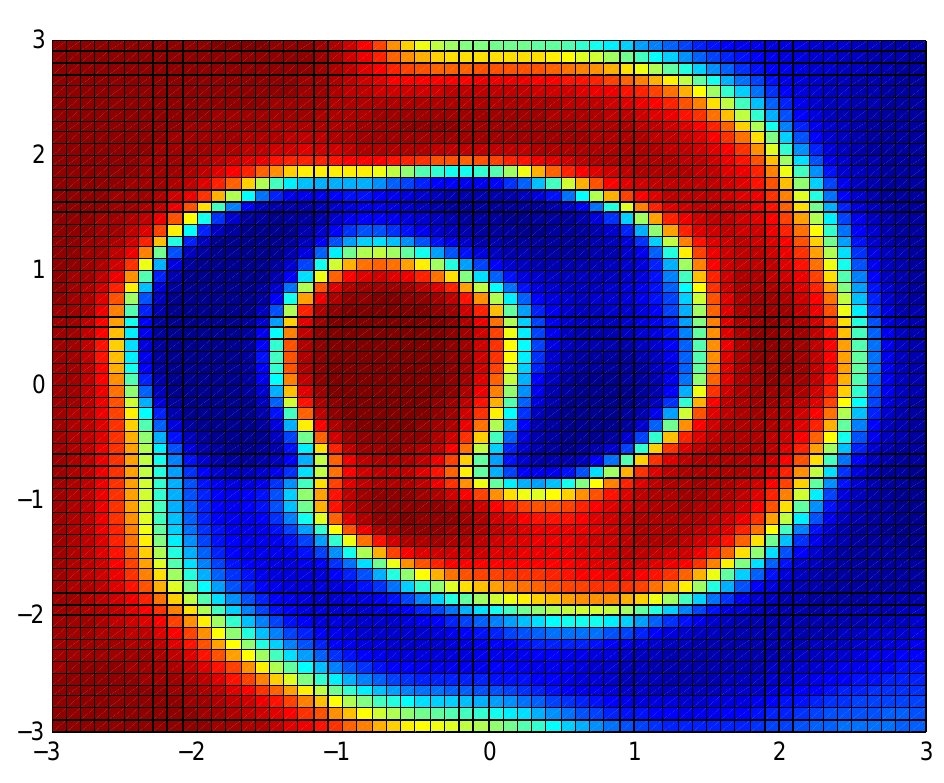
\includegraphics[width=.35\textwidth]{batch_result}
}
\subfigure{
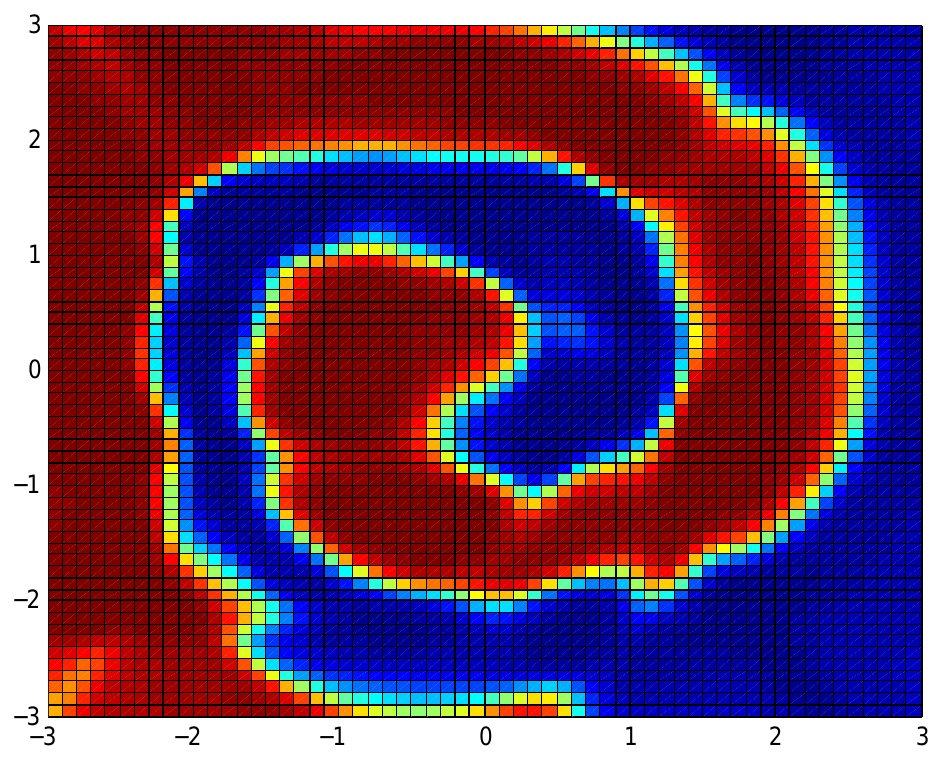
\includegraphics[width=.35\textwidth]{seq_result}
}

\caption{Batch result(left) and Online result(right)}
\label{fig:result}
\end{figure}

\subsection*{3.2 Efficiency}
  \paragraph{} Although the results are both correct, the online learning is more efficient according to my test result.
  The learning rate in batch mode should be much larger than online learning. I don't why. And I have tried many learning rate,
  the total epochs of batch mode is 10 times  more than online learning. 

\begin{figure}[h!]
      \centering
      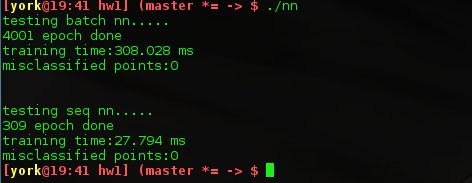
\includegraphics{running_time}
      \caption{Running time comparison}
      \end{figure}
      
      
 

\end{document} 
